\documentclass{standalone}
\usepackage{tikz-cd}
\usepackage{tikz}

\newcommand*{\xMin}{0}%
\newcommand*{\xMax}{4}%
\newcommand*{\yMin}{0}%
\newcommand*{\yMax}{4}%
\begin{document}
	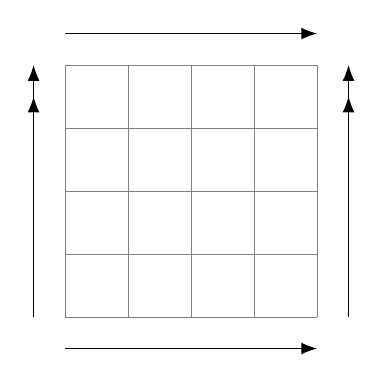
\begin{tikzpicture}[scale=.8]
	\draw[-{Latex[length=2mm]}] (-.5,\yMin)--(-.5,\yMax);
	\draw[-{Latex[length=2mm]}] (-.5,\yMin)--(-.5,\yMax-.5);
	\draw[-{Latex[length=2mm]}] (4.5,\yMin)--(4.5,\yMax);
	\draw[-{Latex[length=2mm]}] (4.5,\yMin)--(4.5,\yMax-.5);
	
	\draw[-{Latex[length=2mm]}] (\xMin, -.5)--(\xMax, -.5);
	\draw[-{Latex[length=2mm]}] (\xMin, 4.5)--(\xMax, 4.5);
	
	\foreach \i in {\xMin,...,\xMax} {
		\draw [very thin,gray] (\i,\yMin) -- (\i,\yMax);
	}
	\foreach \i in {\yMin,...,\yMax} {
		\draw [very thin,gray] (\xMin,\i) -- (\xMax,\i);
	}
	\end{tikzpicture}
\end{document}